\documentclass{article}
\usepackage[utf8]{inputenc}
% Better font encoding for French and scalable fonts
\usepackage[T1]{fontenc}
\usepackage{lmodern}
\usepackage{amsmath, amssymb, amsfonts, amsthm, stmaryrd}
\usepackage{graphicx}
\usepackage{booktabs}
\usepackage{geometry}
\usepackage[french]{babel}
\usepackage{amsopn}

\title{Détection et classification de manoeuvres GEO par apprentissage supervisé : le dataset SPLID - draft}
\author{Etienne Chevrolat}
\date{}


\begin{document}

\maketitle

\begin{abstract}
    On rend compte du travail effectué sur le dataset SPLID (MIT ArcLab) dans le but d'obtenir des modèles de détection de manoeuvres par une approche supervisé. Cinq architectures de détection de manoeuvres inspirées de l'architecture gagnante du {MIT ARCLab Prize for AI Innovation in Space 2024}.

    Le meilleur modèle est un CNN purement convolutif à backbone dupliqué par direction (\texttt{cnn\_split}), doté d'une fenêtre d'entrée asymétrique (128 pas passés, 32 futurs). Il atteint en validation un $F_2$ de $0{,}920$ en détection de noeuds et $0{,}896$ sur la chaîne complète détection + classification, la classification des noeuds étant quasi parfaite ($99{,}5\%$ sur le type de noeud, $99{,}0\%$ sur le type de propulsion).
    Sur le jeu de test officiel du concours, en revanche, le score retombe à $0{,}724$ / $0{,}675$ : qui s'explique par un décalage de distribution entre les jeux d'entraînement et de test.

    Enfin, nous caractérisons quantitativement la raison de l'échec de l'inférence sur les TLE réels de SpaceTrack : SPLID fournit les \emph{éléments osculateurs} de trajectoires \emph{simulées}, échantillonnés régulièrement, là où les TLE sont des \emph{éléments moyens} mesurés à cadence irrégulière — deux domaines de données incompatibles.
\end{abstract}

\section{Le dataset SPLID et la tâche}

\subsection{Structure du dataset}

Le dataset SPLID (\textit{Satellite Pattern-of-Life Identification Dataset}) caractérise le Pattern of Life (PoL) de satellites GEO par une suite de noeuds (points de rupture) séparant des \textit{behavioral modes} (modes de comportement constants entre deux noeuds).
Nous utilisons le jeu \texttt{phase\_2}, celui du concours : \textbf{1900 objets d'entraînement} et \textbf{501 objets de test}, chacun décrit par une série temporelle de 2172 pas de temps à cadence fixe de 2\,h (soit environ 6 mois), contenant les éléments orbitaux osculateurs, les positions géographiques et l'état cartésien du satellite.

\vspace{0.3cm}
\noindent\fbox{%
\begin{minipage}{0.98\textwidth}
\textbf{Labels SPLID}
\begin{itemize}
    \item \textbf{Noeuds} : SS (début de période d'étude), ID (\textit{Initiate Drift}), AD (\textit{Adjust Drift}), IK (\textit{Initiate station-Keeping}), ES (fin de période d'étude) ;
    \item \textbf{Types (modes)} : NK (pas de maintien à poste), CK / EK / HK (maintien à poste chimique / électrique / hybride) ;
    \item \textbf{Directions} : chaque noeud est labellisé Est-Ouest (EW, manoeuvres \textit{in plane}) et/ou Nord-Sud (NS, manoeuvres \textit{out of plane}).
\end{itemize}
Le jeu d'entraînement contient \textbf{5360 noeuds de manoeuvre} (2169 IK, 1812 ID, 1379 AD) et 3800 noeuds SS.
\end{minipage}
}
\vspace{0.3cm}

\subsection{La métrique de performance}

Le concours évalue une soumission (liste de noeuds prédits par objet, avec direction, type de noeud et type de propulsion) par appariement aux noeuds vrais avec une \textbf{tolérance de $\pm 6$ pas de temps} (12\,h), par objet et par direction. Un noeud apparié est un TP si son type de noeud \emph{et} son type de propulsion sont corrects, un FP sinon ; les prédictions non appariées sont des FP et les noeuds vrais manqués des FN. Le score agrégé est le
$$
F_2 = \dfrac{5\,TP}{5\,TP + 4\,FN + FP}
$$
qui favorise le rappel (il vaut mieux sur-détecter que manquer une manoeuvre), complété par le RMSE des écarts temporels des TP.


\section{Recréation de la pipeline de données}

Toute la pipeline, des fichiers CSV bruts aux tenseurs PyTorch, a été recréée dans le repo global de travail \texttt{ssa-analysis/}.

\vspace{0.3cm}
\noindent\fbox{%
\begin{minipage}{0.98\textwidth}
\textbf{Pipeline localizer (détection)}
\begin{enumerate}
    \item \textbf{Features continues} : les éléments angulaires discontinus $(e, i, \Omega, \omega, \nu)$ sont convertis en éléments équinoxiaux continus $(k, h, q, p, \cos\lambda, \sin\lambda)$, ce qui évite les sauts $360^\circ \to 0^\circ$ ;
    \item \textbf{Dérivées discrètes} : on ajoute les incréments $\Delta a$, $\Delta q$, $\Delta p$ entre pas consécutifs, qui portent la signature impulsionnelle des manoeuvres, soit 9 features au total ;
    \item \textbf{Normalisation} : standardisation ajustée sur le train uniquement ;
    \item \textbf{Cibles} : deux canaux (EW, NS) valant des bosses triangulaires de demi-largeur 6 pas centrées sur les noeuds de manoeuvre, à zéro ailleurs ;
    \item \textbf{Fenêtrage} : chaque exemple est une fenêtre glissante de $N$ pas ($N_p$ passés, $N_f$ futurs) centrée sur l'instant à prédire, soit un tenseur $(9, N)$ ;
    \item \textbf{Split} : 80/20 \emph{par objet} (1520 objets train, 380 objets validation), pour éviter toute fuite entre train et validation.
\end{enumerate}
\end{minipage}
}
\vspace{0.3cm}

Le \textbf{classifier} réutilise les mêmes features et fenêtres, mais échantillonnées uniquement aux instants des noeuds labellisés ; il prédit deux sorties par fenêtre : le type de noeud (ID/AD/IK) et le type de propulsion (NK/CK/EK/HK), avec une pondération de classes compensant le déséquilibre.

\section{Modèles}

Cinq architectures de localizer ont été réimplémentées et comparées, à features identiques :

\begin{itemize}
    \item \texttt{naive\_baseline} : une simple couche linéaire sur la fenêtre aplatie (calibre le problème) ;
    \item \texttt{small\_cnn} : 3 couches de convolution 1D (64, 64, 48 canaux, noyaux 7) + tête dense ;
    \item \texttt{small\_lstm} : une couche LSTM (32 unités) + max-pooling temporel + tête dense ;
    \item \texttt{cnn\_lstm1} : \textbf{CNN et LSTM en série} : les 3 couches de convolution extraient les motifs locaux et compressent l'axe temporel ($97 \to 40$), puis un LSTM (64 unités) agrège séquentiellement, suivi d'un max-pooling et d'une tête dense à 2 sorties (probabilité d'un noeud EW / NS au centre de la fenêtre) ;
    \item \texttt{cnn\_split} : \textbf{CNN pur à backbone dupliqué par direction}.
\end{itemize}

\section{Résultats}

\subsection{Comparaison des architectures}

Courbes de validation des localizers (loss BCE et $F_2$ à seuil de détection fixe de $0{,}1$) :

\begin{center}
    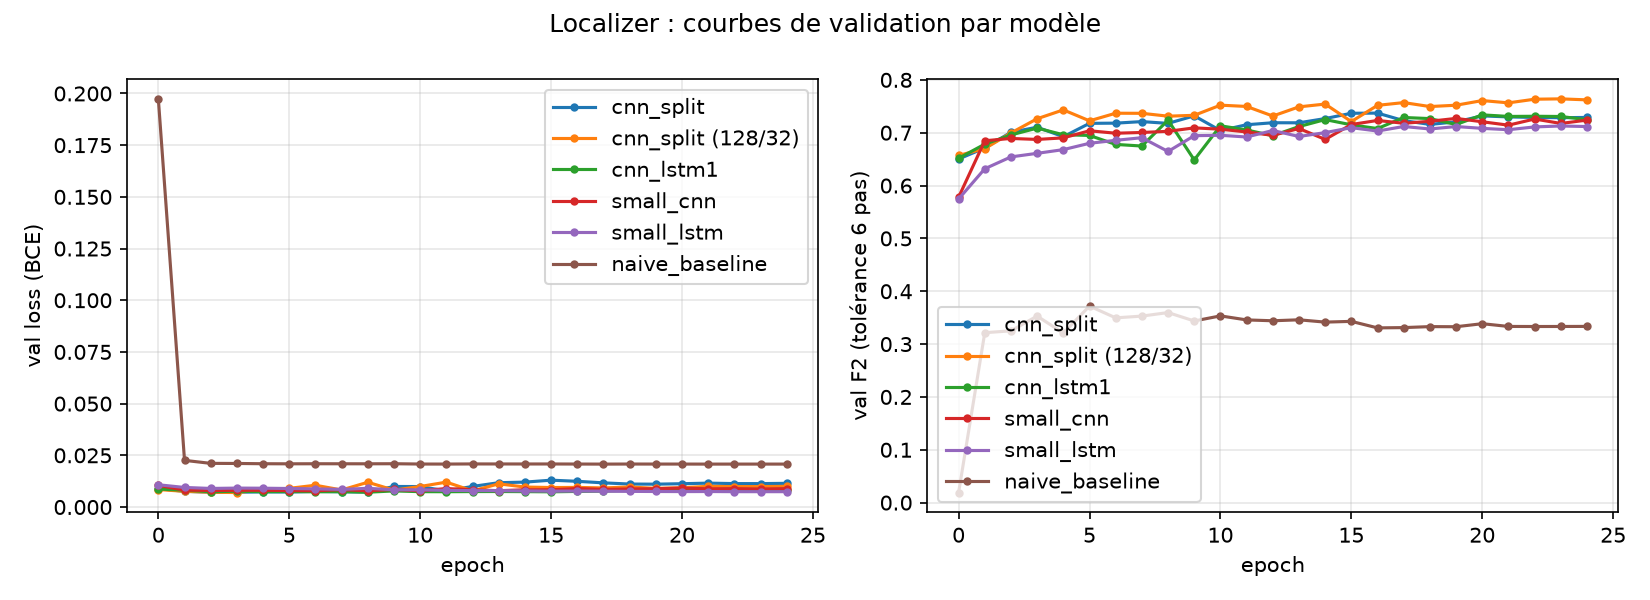
\includegraphics[width=0.98\textwidth]{figures/splid_training_curves.png}
\end{center}

\begin{center}
\begin{tabular}{llc}
\toprule
Modèle & Fenêtre & $F_2$ max en validation (seuil $0{,}1$) \\
\midrule
naive\_baseline & 48/48 & 0,372 \\
small\_lstm & 48/48 & 0,713 \\
small\_cnn & 48/48 & 0,727 \\
cnn\_lstm1 (série) & 48/48 & 0,734 \\
cnn\_split & 48/48 & 0,741 \emph{et} 0,737 \\
\textbf{cnn\_split} & \textbf{128/32} & \textbf{0,764} \\
\bottomrule
\end{tabular}
\end{center}


\subsection{L'écart entre les deux directions}

Le score global masque une asymétrie forte entre les deux directions. Nous mesurons donc chaque architecture direction par direction, chacune à son propre seuil optimal, afin que la comparaison ne dépende pas d'un seuil global favorisant la direction dominante :

\begin{center}
    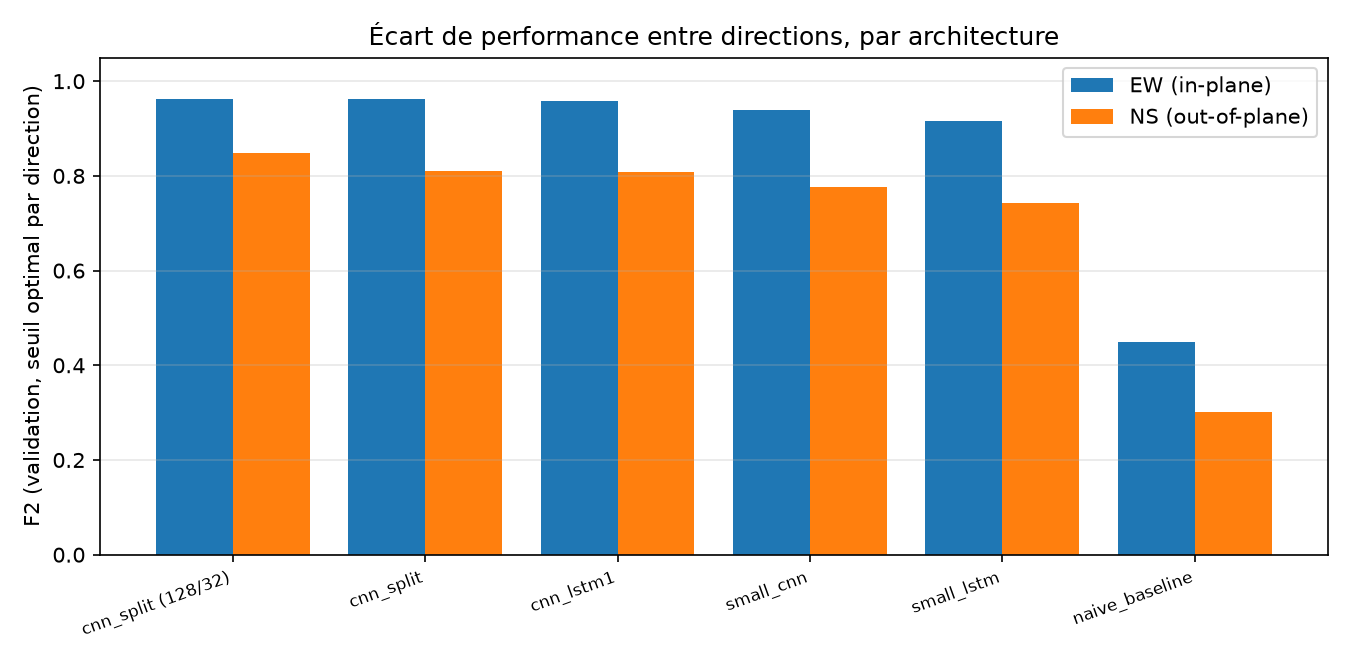
\includegraphics[width=0.95\textwidth]{figures/splid_per_direction.png}
\end{center}

Trois enseignements se dégagent  :

\paragraph{La détection NS est systématiquement le maillon faible.} Quelle que soit l'architecture, le $F_2$ NS accuse $0{,}12$ à $0{,}17$ de retard sur le $F_2$ EW. Le déficit porte sur le \emph{rappel} (les manoeuvres out-of-plane sont manquées, non sur-détectées), et non sur la précision.

\paragraph{Le backbone dupliqué ne corrige pas cet écart.} À fenêtre égale, \texttt{cnn\_split} obtient $0{,}810$ en NS contre $0{,}808$ pour \texttt{cnn\_lstm1} : la séparation des deux branches, qui devait précisément éviter qu'un backbone commun sacrifie la direction minoritaire, ne change rien de mesurable. L'hypothèse d'un compromis imposé par le partage de paramètres n'est donc pas ce qui limitait la détection NS.

\paragraph{C'est le contexte passé qui compte.} Tout le gain NS provient de l'allongement de la fenêtre ($0{,}810 \to 0{,}849$, rappel $0{,}799 \to 0{,}853$), à architecture inchangée. Passer de 4 à 10,7 jours de contexte passé donne au réseau de quoi estimer le changement de pente dans l'inclinaison de part et d'autre du noeud.

\subsection{Choix du seuil de détection}

La sortie du localizer est une probabilité par pas de temps ; les noeuds prédits sont les centres des plages au-dessus d'un seuil. Ce seuil arbitre précision contre rappel. Les comptages TP/FP/FN s'additionnant entre directions, nous les tabulons une fois par direction et par seuil, puis cherchons le couple $(\text{seuil EW}, \text{seuil NS})$ optimal sur la grille :

\begin{center}
    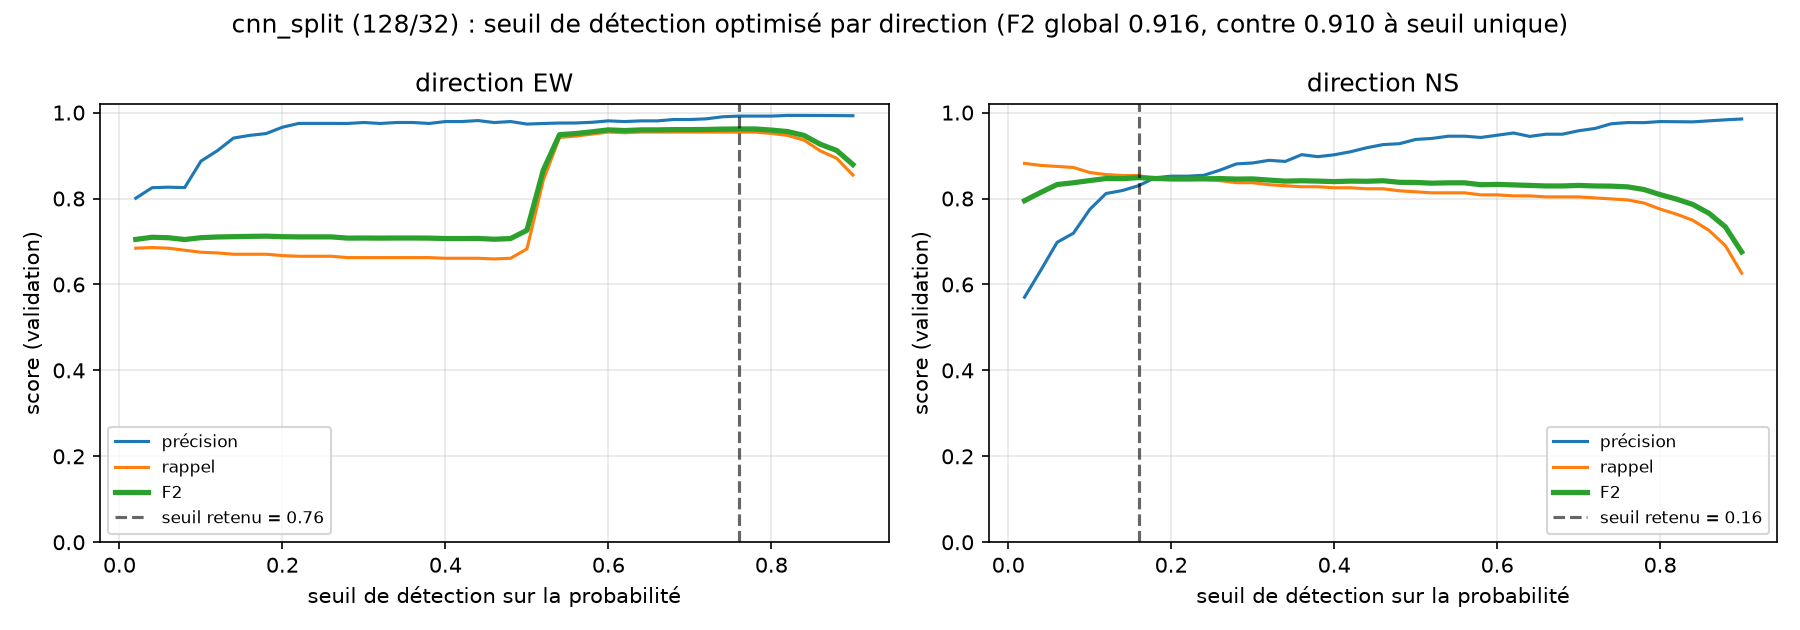
\includegraphics[width=0.98\textwidth]{figures/splid_threshold_sweep.png}
\end{center}

Le seuil optimal est très différent d'une direction à l'autre : $0{,}76$ en EW contre $0{,}16$ en NS. Cet écart est une mesure directe de l'asymétrie décrite plus haut, le réseau est franchement confiant sur les noeuds EW, où il produit des pics de probabilité nets, et beaucoup plus timide sur les noeuds NS.

Relever le seuil au-delà du défaut de $0{,}1$ apporte en revanche un gain net ($F_2$ passant de $0{,}764$ à $0{,}916$) : le modèle produit des pics francs, et remonter le seuil élimine beaucoup de fausses alarmes de faible amplitude sans coûter de rappel.


C'est une différence de fond avec les méthodes par seuillage de résidus (filtre de Kalman, cf. rapport précédent) : le seuil s'applique ici à une probabilité apprise, homogène d'un satellite à l'autre, et non à une grandeur physique dont l'échelle varie selon l'objet. Il se règle donc \emph{une seule fois} pour tout le catalogue, 
ce qui lève l'obstacle principal à l'automatisation qui était la recherche d'un seuil optimal sans plus d'informations

\subsection{Score officiel en validation}

Évaluateur officiel du concours sur les 380 objets de validation :

\begin{center}
\begin{tabular}{lcccc}
\toprule
 & Précision & Rappel & $F_2$ & RMSE (pas) \\
\midrule
Détection seule (ID/AD/IK) & 0,945 & 0,914 & \textbf{0,920} & 0,54 \\
Chaîne complète (mode concours) & 0,761 & 0,938 & \textbf{0,896} & 0,41 \\
\bottomrule
\end{tabular}
\end{center}

En détection seule : 972 TP pour seulement 57 FP et 91 FN. Le RMSE de $0{,}54$ pas signifie que les noeuds détectés sont localisés à moins de $1{,}1$\,h de la manoeuvre vraie en moyenne — une précision temporelle très supérieure à la tolérance de 12\,h.

\subsection{Score sur le jeu de test officiel}

Le seuil ayant été calibré sur la validation, 
nous l'appliquons tel quel aux 501 objets de test officiels, jamais vus :

\begin{center}
\begin{tabular}{lcccc}
\toprule
 & Précision & Rappel & $F_2$ & RMSE (pas) \\
\midrule
Détection seule (ID/AD/IK) & 0,901 & 0,690 & 0,724 & 0,49 \\
Chaîne complète (mode concours) & 0,423 & 0,793 & 0,675 & 0,33 \\
\bottomrule
\end{tabular}
\end{center}

\textbf{À comparer au gagnant du concours, qui obtient $F_2 = 0{,}805$ 
sur ce même jeu de test en chaîne complète : nous sommes en deçà ($0{,}675$).} 

\paragraph{Un décalage de distribution des labels.} 
La distribution des types de propulsion diffère fortement entre les deux jeux :

\begin{center}
\begin{tabular}{lcccc}
\toprule
Type de propulsion (noeuds SS) & NK & CK & EK & HK \\
\midrule
Entraînement (3800 noeuds) & 55\,\% & 22\,\% & 19\,\% & 4\,\% \\
Test (1000 noeuds) & 26\,\% & 27\,\% & 32\,\% & 15\,\% \\
\bottomrule
\end{tabular}
\end{center}

Le jeu de test est donc bien plus riche en propulsion électrique (EK) et hybride (HK), i.e.  les régimes à poussée faible et prolongée, 
De plus, tout l'entrainement a été fait en excluant les noeuds artificiels SS et ES pour ne privilégier que des noeuds de POL réels, donc ce score décevant n'est pas vraiment à prendre en compte.
\subsection{Exemples qualitatifs}

Pour trois objets de validation parmi les plus manoeuvrants : demi-grand axe, inclinaison, et sortie du localizer, superposés aux labels (traits verticaux, EW en bleu, NS en orange pointillé).

\begin{center}
    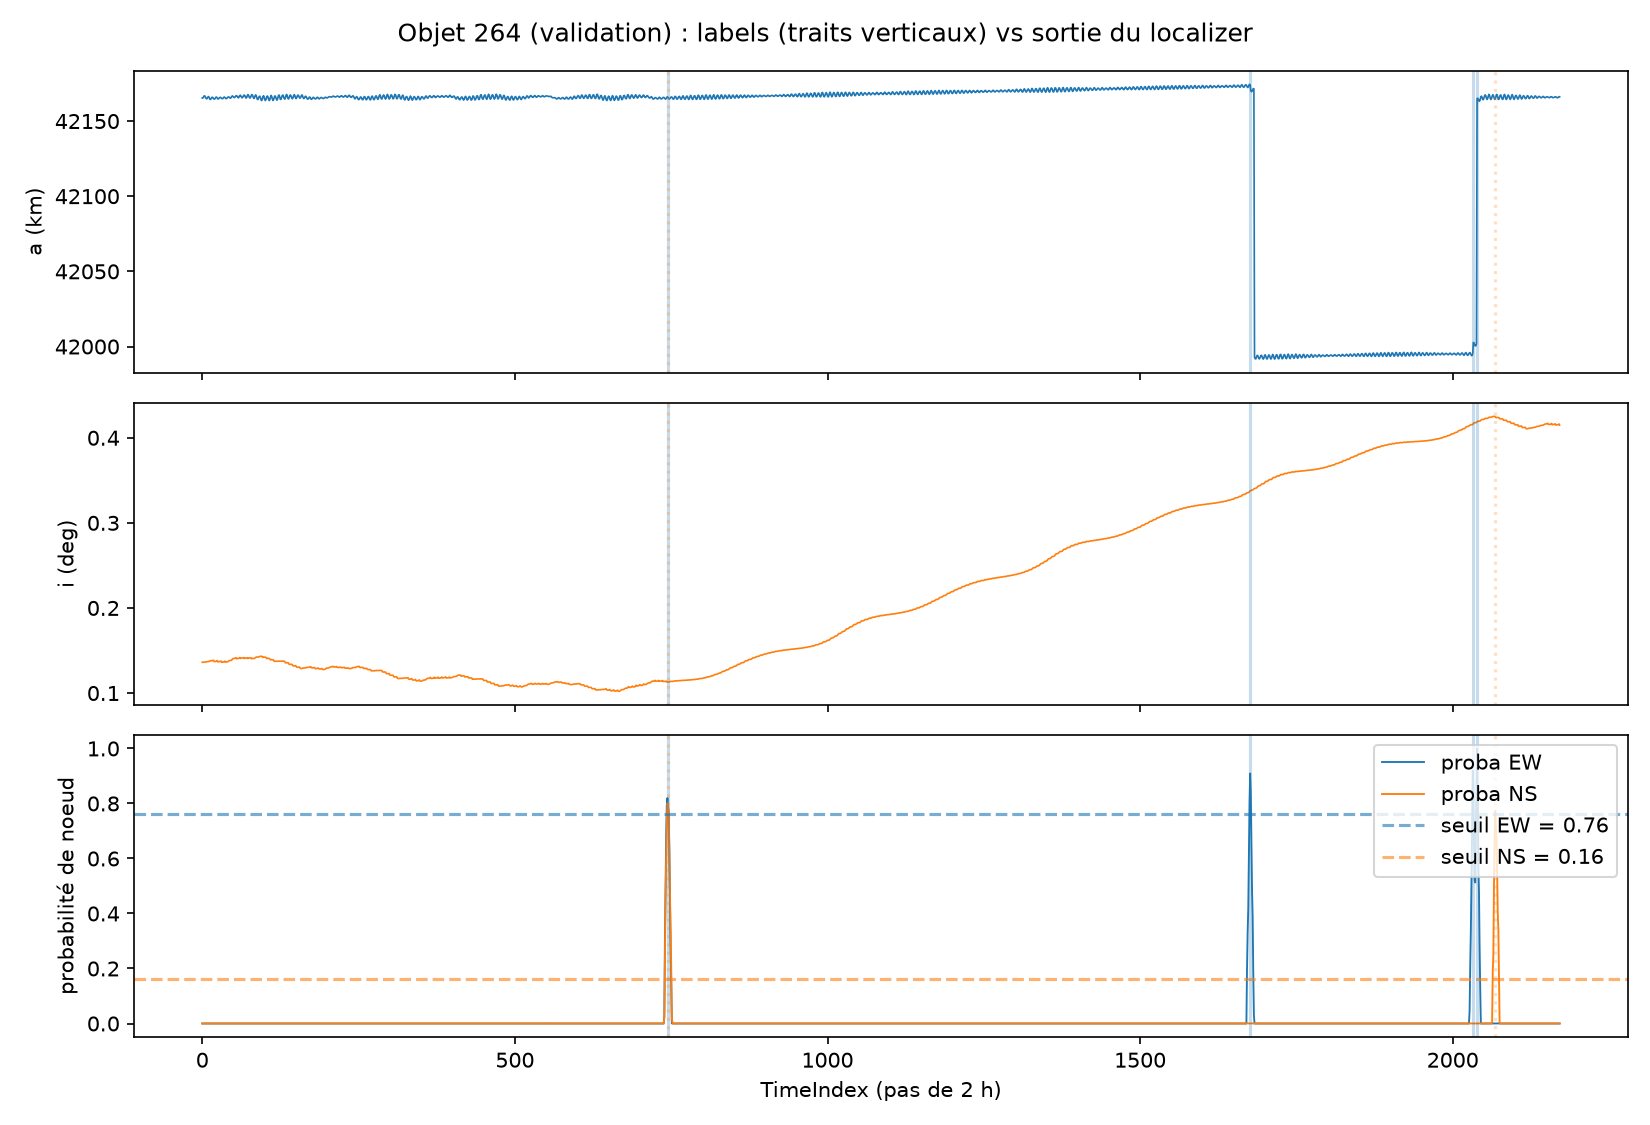
\includegraphics[width=0.95\textwidth]{figures/splid_example_264.png}
\end{center}
\begin{center}
    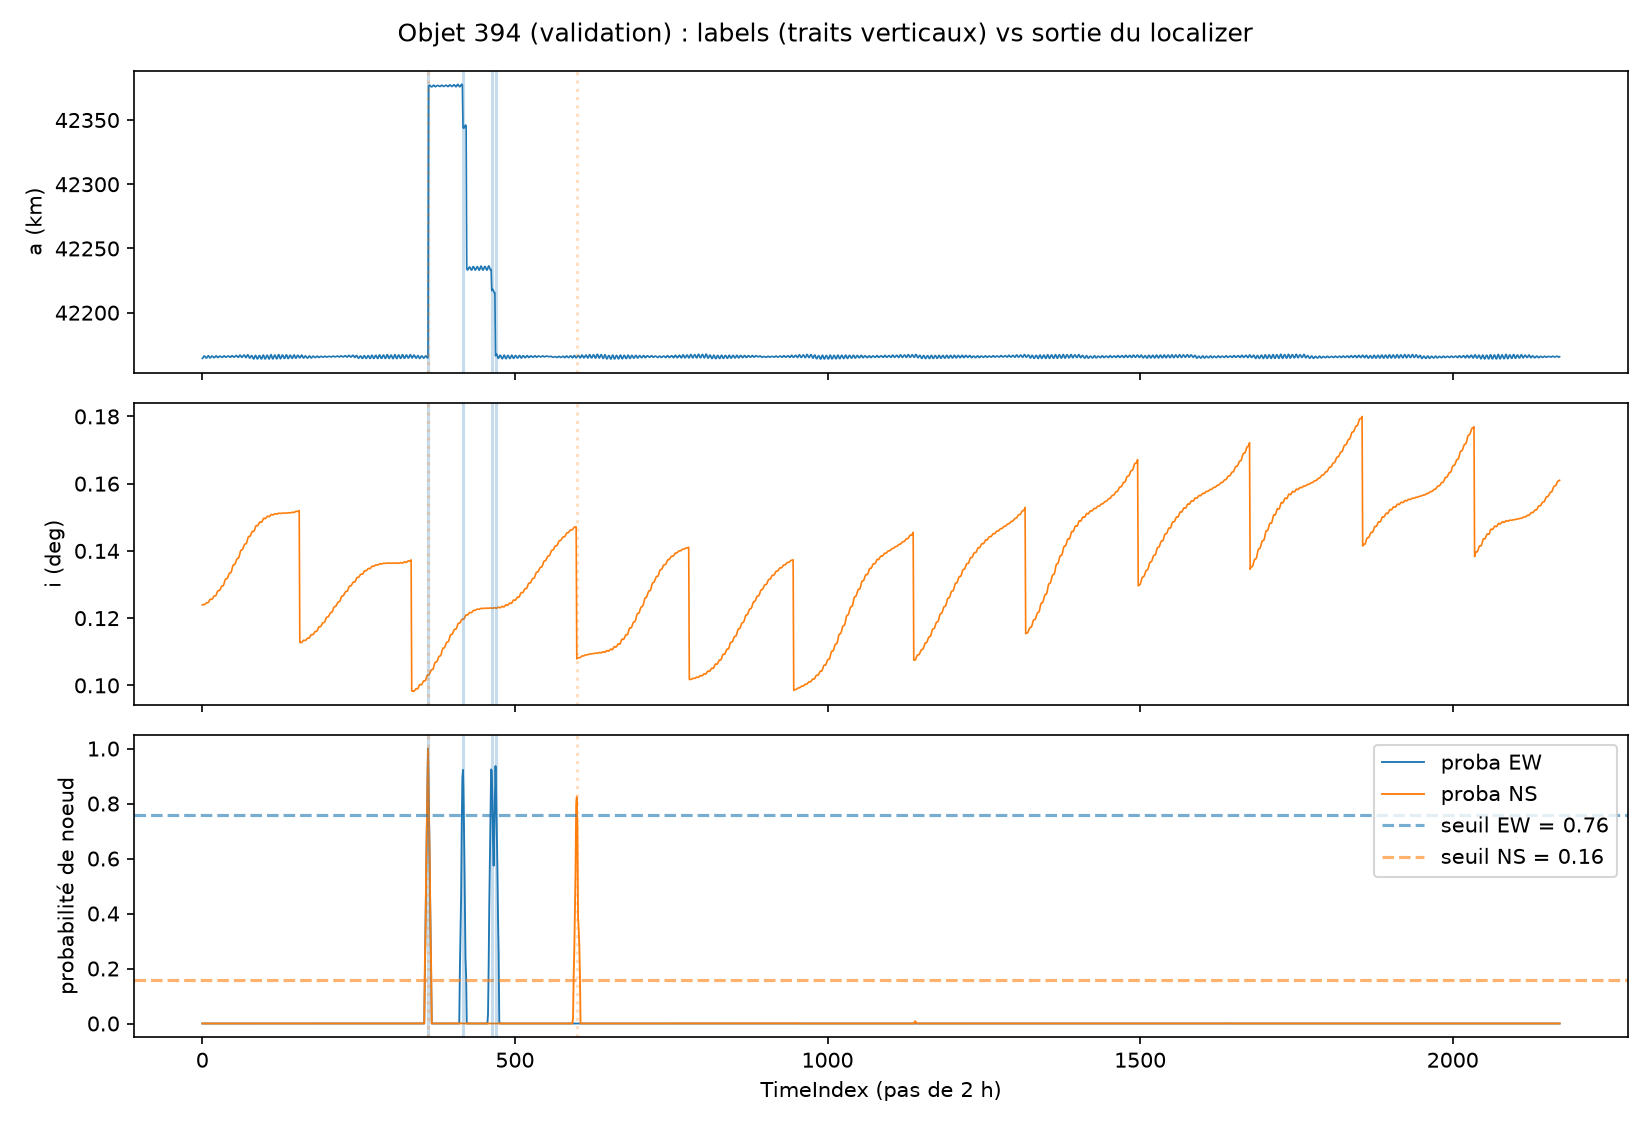
\includegraphics[width=0.95\textwidth]{figures/splid_example_394.png}
\end{center}
\begin{center}
    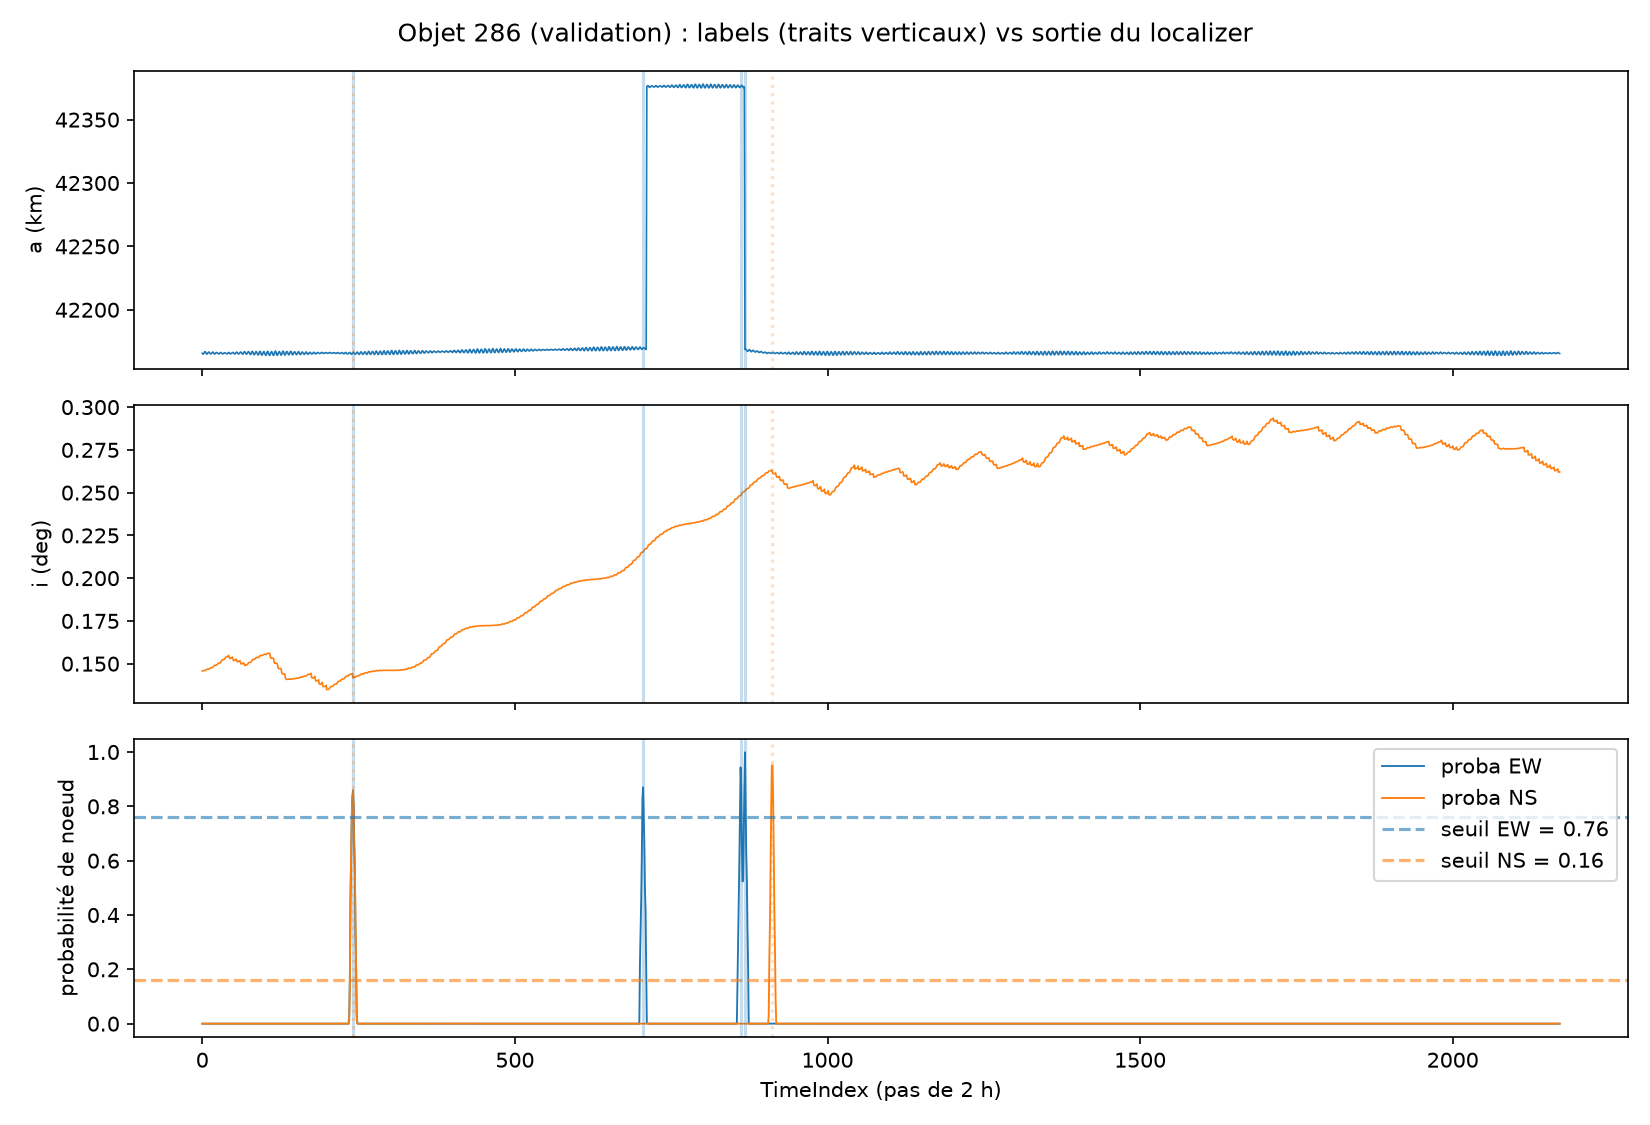
\includegraphics[width=0.95\textwidth]{figures/splid_example_286.png}
\end{center}

Les pics de probabilité sont remarquablement francs et coïncident avec les manoeuvres EW (visibles comme des sauts du demi-grand axe) comme avec les manoeuvres NS (ruptures de pente de l'inclinaison), y compris lorsque ces dernières sont difficiles à repérer à l'oeil nu.

\subsection{Classification des noeuds}

Le classifier \texttt{cnn\_lstm1} sur les noeuds de validation :

\begin{center}
    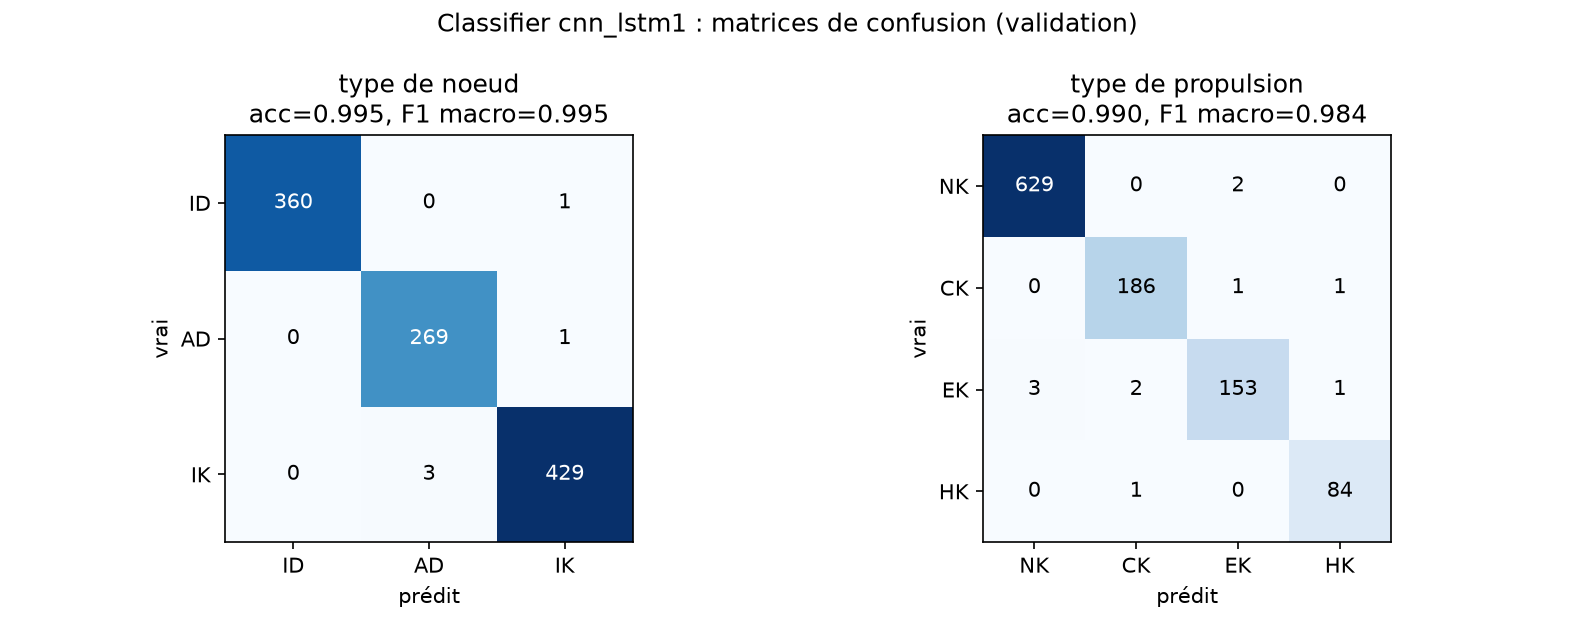
\includegraphics[width=0.9\textwidth]{figures/splid_classifier_confusion.png}
\end{center}

La classification est quasi parfaite en validation : $99{,}5\%$ d'exactitude sur le type de noeud (5 erreurs sur 1063) et $99{,}0\%$ sur le type de propulsion. Les signatures des différents régimes (CK : impulsions fortes et espacées ; EK/HK : poussées faibles quasi continues) sont donc parfaitement séparables par le réseau — \emph{lorsque la distribution d'entraînement couvre celle d'évaluation}, ce qui n'est plus le cas sur le jeu de test (section précédente).

\section{Le problème du transfert vers SpaceTrack}

L'objectif final reste la détection sur données réelles. Une passe d'inférence des modèles entraînés sur SPLID a donc été menée sur notre historique de TLE SpaceTrack de satellites GEO, remis au format SPLID (renommage des colonnes, ré-interpolation des éléments équinoxiaux sur une grille régulière de 2\,h, découpage aux trous de données). \textbf{Les résultats sont inexploitables}, et l'analyse quantitative des deux domaines montre que ce n'est pas un problème d'architecture ni d'entraînement, mais d'incompatibilité de la nature même des données.

\begin{center}
    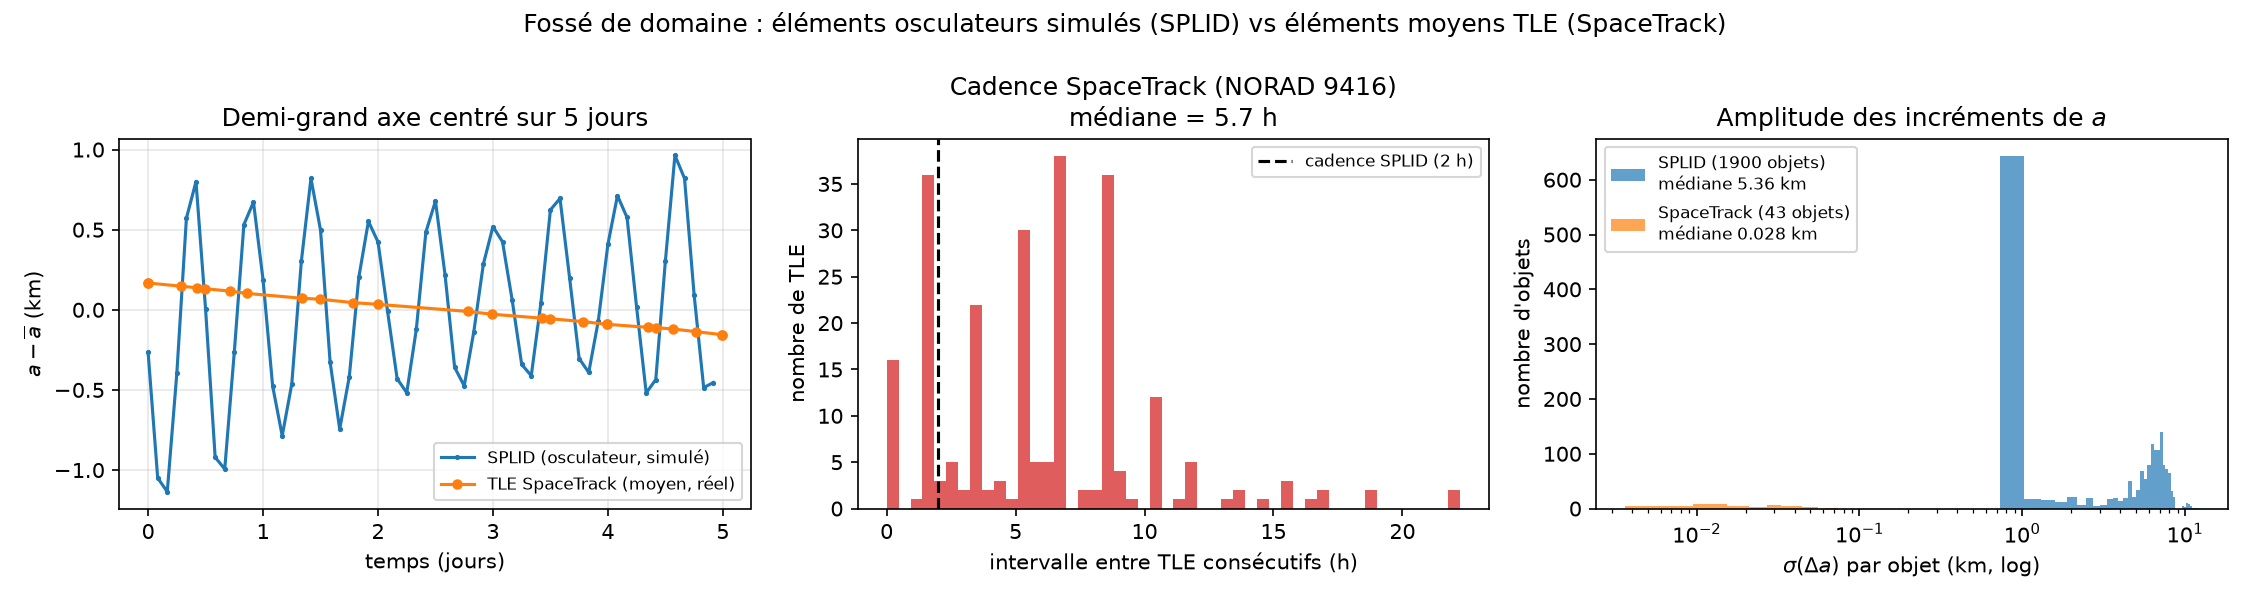
\includegraphics[width=0.98\textwidth]{figures/splid_domain_gap.png}
\end{center}

\paragraph{Éléments osculateurs contre éléments moyens.} C'est le point central. La documentation du dataset l'indique explicitement : SPLID fournit les \emph{éléments orbitaux osculateurs} de trajectoires produites par un simulateur haute fidélité. Le demi-grand axe y porte donc les oscillations à courte période (12\,h et 24\,h en GEO, dues aux harmoniques du champ terrestre), d'amplitude crête-à-crête de plusieurs kilomètres — parfaitement visibles sur le panneau de gauche.
Les TLE de SpaceTrack sont au contraire des \emph{éléments moyens} au sens SGP4 : ces termes à courte période en ont été analytiquement retirés, et la série est lisse.
Quantitativement, l'écart-type des incréments $\Delta a$ entre échantillons successifs, qui est l'une des features principales du modèle, vaut en médiane :
$$
\sigma(\Delta a)_{\text{SPLID}} = 5{,}36~\text{km} \qquad \text{contre} \qquad \sigma(\Delta a)_{\text{SpaceTrack}} = 0{,}028~\text{km},
$$
soit un rapport de près de \textbf{200}. La composante dominante de la variance des features apprises n'existe tout simplement pas dans les TLE.

\paragraph{Cadence d'échantillonnage.} SPLID est échantillonné exactement toutes les 2\,h. Les TLE arrivent à intervalles irréguliers, de médiane $5{,}7$\,h pour le satellite GEO représenté, avec une queue au-delà de 20\,h. La ré-interpolation sur une grille de 2\,h fabrique donc de longues plages artificiellement lisses entre deux TLE, sans équivalent dans les données d'entraînement.

\paragraph{Données simulées contre données mesurées.} Enfin, les trajectoires SPLID d'entraînement sont simulées, donc exemptes du bruit d'estimation propre aux TLE, qui résultent d'un ajustement sur observations radar et optiques.

Le modèle apprend donc des signatures fines dans des séries propres, régulières et riches en oscillations à courte période — signatures qui n'existent pas sous cette forme dans les TLE réels. C'est un \textit{domain gap} au sens strict.

\section{A suivre}
\begin{itemize}
    \item La pipeline SPLID est complète, reproductible et évaluée avec la métrique officielle du concours, sur le jeu d'entraînement comme sur le jeu de test : elle constitue un banc d'essai fiable pour itérer sur les architectures ;
    \item les performances en validation ($F_2 = 0{,}920$ en détection, classification des noeuds à $99\%$) montrent que l'approche par fenêtre glissante apprend effectivement les signatures de manoeuvres, et que le seuil de détection y est réglable une fois pour toutes — deux propriétés que les méthodes par filtrage de Kalman n'offraient pas ;
    \item l'écart à notre score de test ($0{,}675$ contre $0{,}805$ pour le gagnant) n'est pas vraiment à prendre en compte car on n'a pas considéré pendant l'entrainement des noeuds SS et ES (les scores sont donc faussés)
    \item pour les données réelles, le transfert direct depuis SPLID est une impasse. Deux pistes : dégrader les données SPLID pour les rapprocher du domaine TLE (passage aux éléments moyens par filtrage des termes à courte période, sous-échantillonnage irrégulier, ajout de bruit d'estimation), et/ou entraîner directement sur des TLE réels labellisés (labels ILRS en LEO, labellisation manuelle en GEO, cf. rapport précédent) ;
    \item le pré-entraînement non supervisé (MAE) sur l'historique massif SpaceTrack est la voie finalement choisie: apprendre des représentations directement dans le domaine des TLE réels.
\end{itemize}

\end{document}